\section{The Mandate: Carbon Rules Closing In From Both Sides}\label{sec:mandate}

\subsection{Taiwan's own laws: net-zero, NDC targets, and the carbon fee}\label{sec:tw}

Taiwan wrote its climate destination into law. The Climate Change Response Act
(2023) makes \textbf{net-zero emissions by 2050 a statutory goal}, and the
government's ``NDC~3.0'' targets, announced in 2025, commit to cuts of
\textbf{28\%$\pm$2\% by 2030, 32\%$\pm$2\% by 2032, and 38\%$\pm$2\% by 2035}
against the 2005 baseline --- among the most ambitious trajectories in
Asia\cite{ndc} (Figure~\ref{fig:ndc}).

\begin{figure}[htbp]
\centering
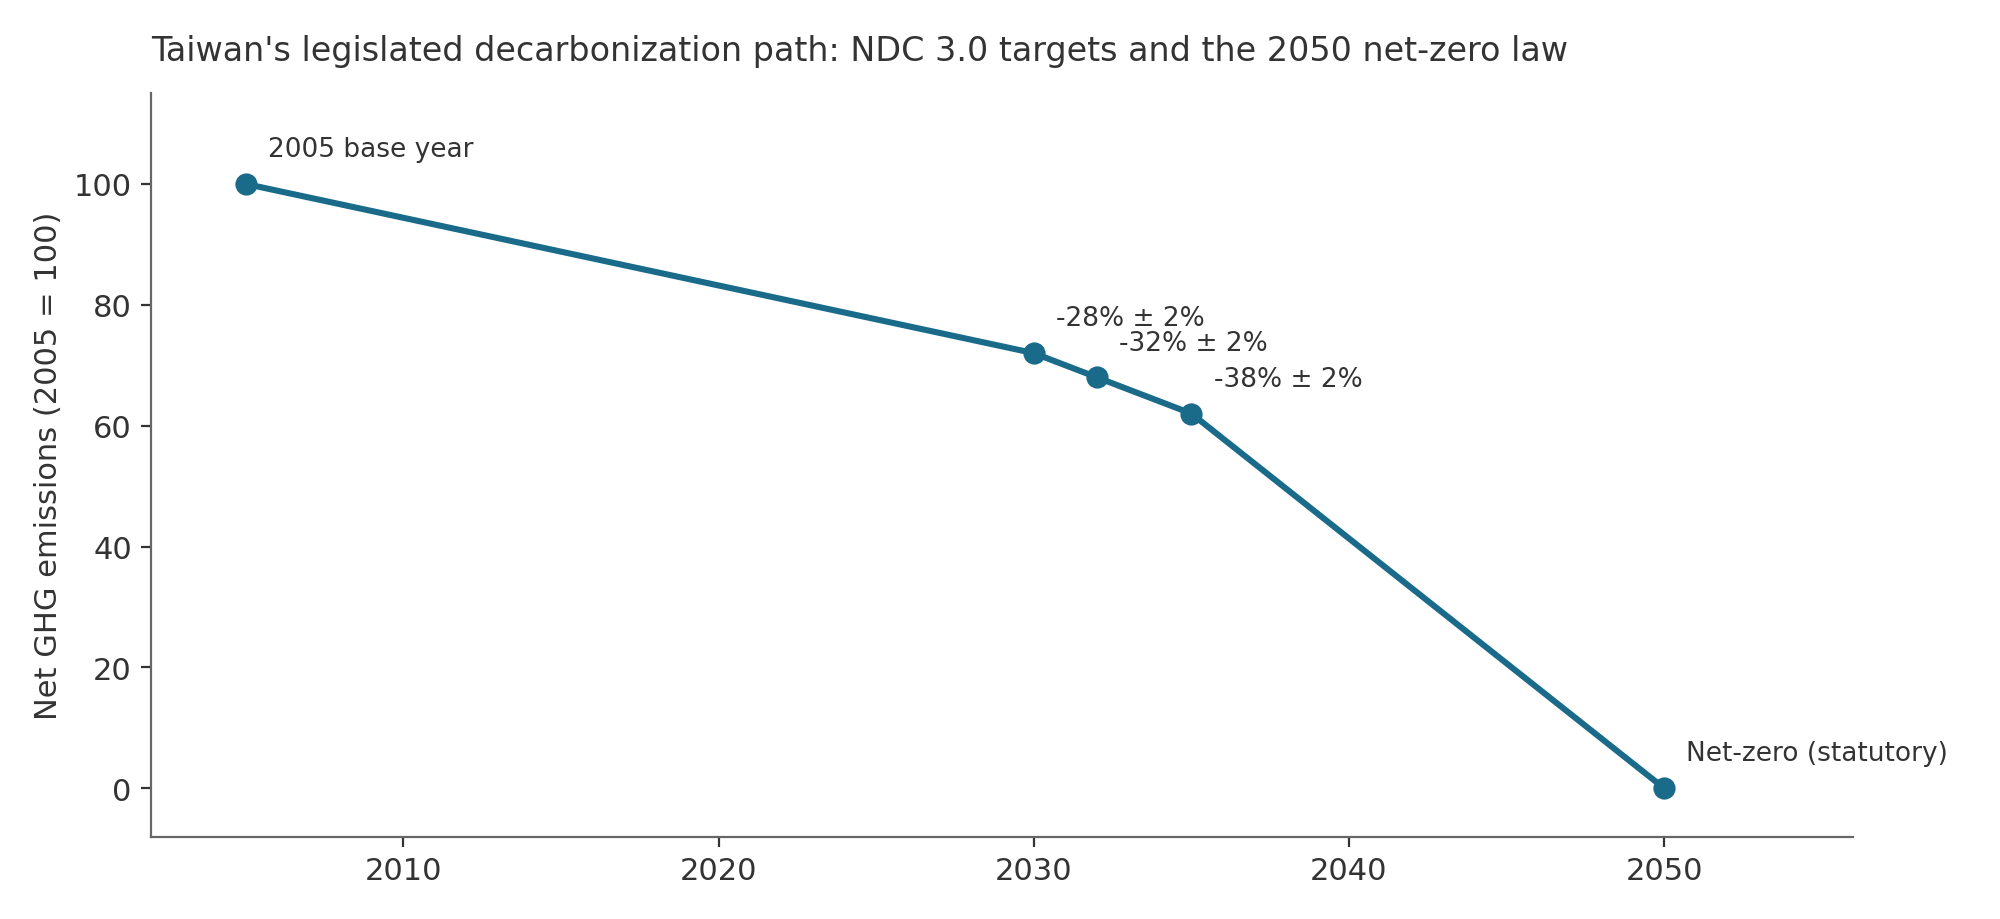
\includegraphics[width=0.95\textwidth]{chart4_ndc.png}
\caption[Taiwan's legislated decarbonization path (NDC 3.0)]{Taiwan's
legislated emissions path: NDC~3.0 targets (MOENV, 2025\cite{ndc}) and the
statutory 2050 net-zero goal.}
\label{fig:ndc}
\end{figure}

The first enforcement instrument is the \textbf{carbon fee}. Firms emitting
more than 25,000~tCO$_2$e per year (Scope~1+2) pay NT\$300 per tonne, reducible
to NT\$100 or NT\$50 if the regulator approves a rigorous ``Self-Determined
Reduction Plan''; industries at high risk of relocating abroad apply a 0.2
adjustment coefficient, an effective floor near NT\$10/t\cite{moenvfee,reset}.
The first collection cycle closed on 31~May~2026 and raised \textbf{NT\$4.97
billion from 461 factories run by 240 companies}\cite{focus,tptfee}
(Figure~\ref{fig:fee}). Tellingly, of $\sim$430 factories that applied for the
discounted rates, about 28 were withdrawn or rejected --- evidence that even
well-resourced corporations struggle to produce reduction plans that survive
regulatory scrutiny\cite{focus}.

\begin{figure}[htbp]
\centering
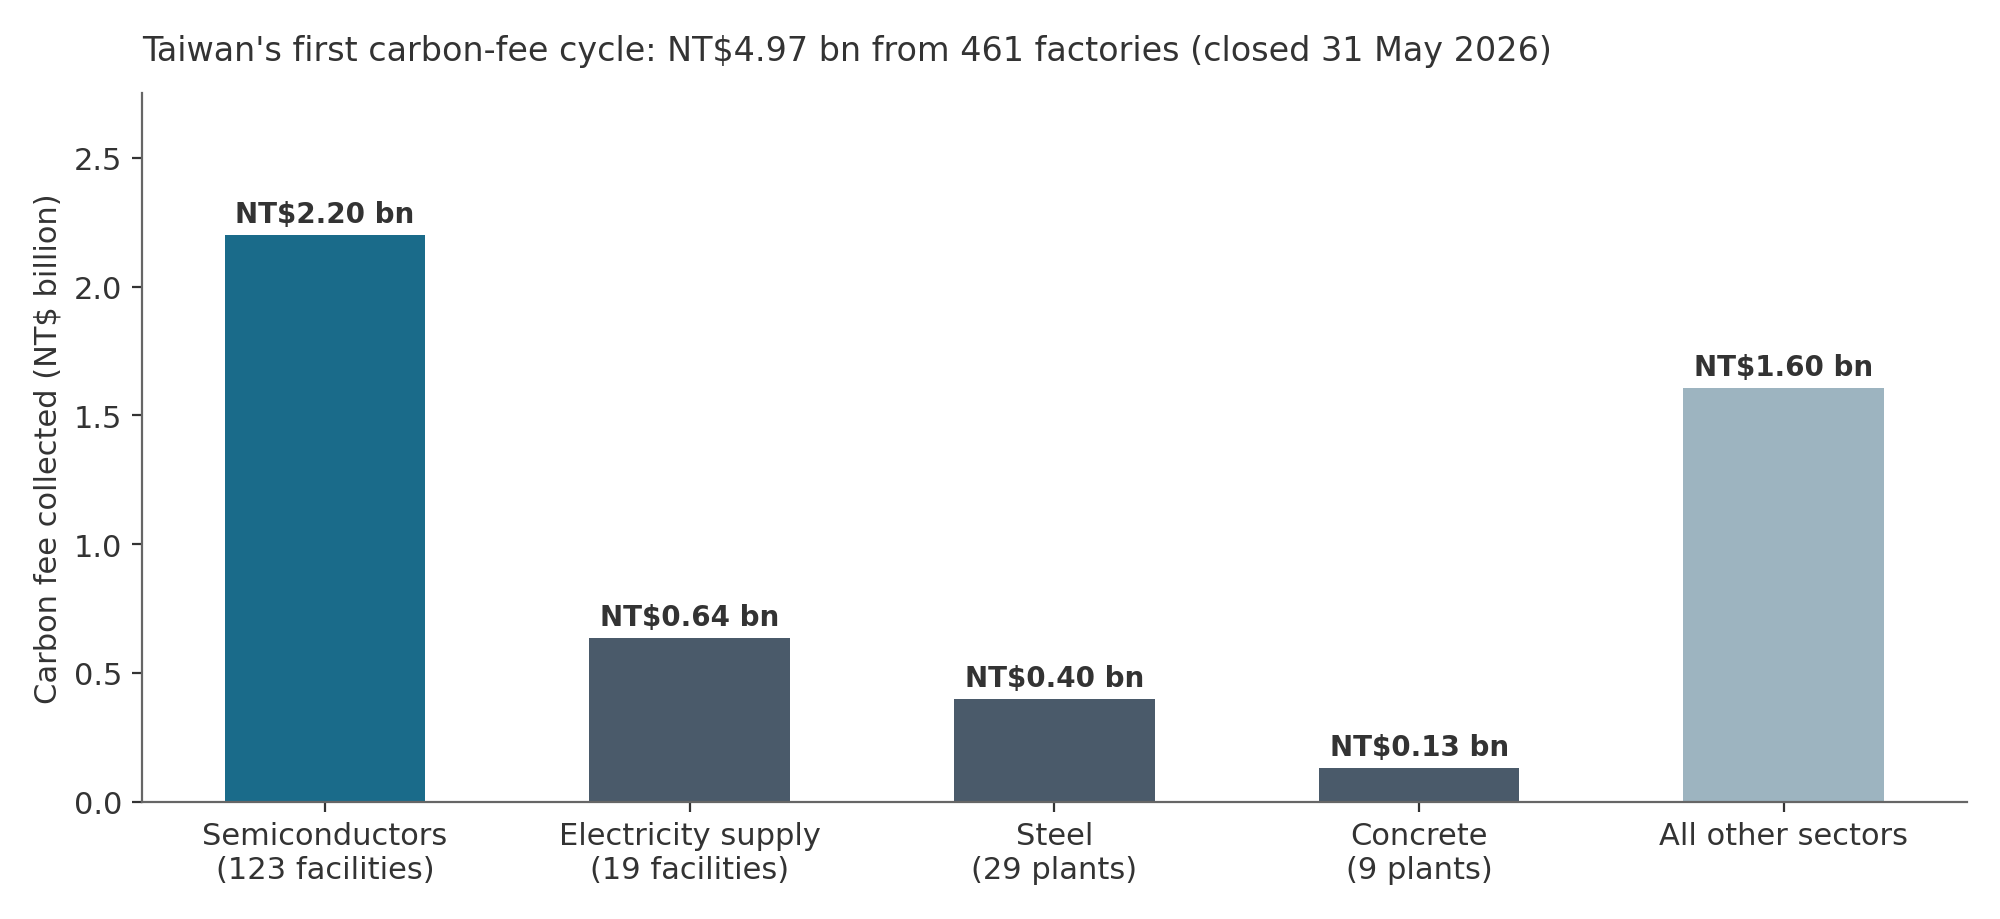
\includegraphics[width=0.95\textwidth]{chart2_fee.png}
\caption[First-cycle carbon-fee revenue by sector]{First-cycle carbon-fee
revenue by sector (MOENV via Focus Taiwan / Taipei Times, June
2026\cite{focus,tptfee}). Semiconductors paid 44\%, including 33 TSMC fabs.}
\label{fig:fee}
\end{figure}

\begin{keyfact}{A correction this proposal carries deliberately.}
Discounted (``preferential'') fee rates depend only on the large emitter's
\emph{own} Scope~1+2 reductions --- not on its suppliers'
data\cite{moenvfee,reset}. Supplier carbon pressure in Taiwan is real, but it
flows from voluntary corporate commitments (SBTi, RE100) and programs such as
TSMC's NT\$5.5\,bn supplier carbon-reduction subsidy scheme\cite{tsmc} --- not
from the fee. Early drafts of this concept got that causal chain wrong; the
corrected version is what appears here.
\end{keyfact}

Three forward signals matter: the 25,000\,t threshold is set to be lowered over
time; fee levels are signalled to rise (potentially NT\$1,200--1,800/t by
2030); and a pilot emissions-trading system is planned around
2027\cite{ecobiz}. Firms outside the fee today will not all stay outside it.

\subsection{The European Union's border carbon price (CBAM)}\label{sec:cbam}

The EU charges its own industries for carbon through the ETS. To stop
production simply relocating to unregulated countries (``carbon leakage''),
CBAM extends that carbon price to imports. Table~\ref{tab:timeline} gives the
timeline that turned this from paperwork into money.

\begin{table}[htbp]
\caption{CBAM timeline and mechanics relevant to Taiwanese exporters}
\label{tab:timeline}
\small
\begin{tabularx}{\textwidth}{@{}p{0.185\textwidth}Xp{0.09\textwidth}@{}}
\toprule
\textbf{Date} & \textbf{What happens} & \textbf{Source} \\
\midrule
Oct 2023 -- Dec 2025 & Transitional phase: EU importers report embedded emissions quarterly; no payment; generic default values broadly permitted & \cite{taxud} \\
Oct 2025 & ``Omnibus'' simplification: 50-tonne annual de minimis exempts $\sim$90\% of importers while retaining $\sim$99\% of covered emissions --- but the threshold is counted \textbf{cumulatively per importer}, so small suppliers can still be swept in & \cite{icap} \\
\textbf{1 Jan 2026} & \textbf{Definitive phase: importers must buy and surrender CBAM certificates.} Certificate price = quarterly EU ETS auction average: \textbf{EUR 75.36 (Q1 2026), EUR 75.28 (Q2 2026)} & \cite{taxud,ecprice} \\
2026--2028 & Default values set at highest observed intensity, marked up +10\% (2026), +20\% (2027), +30\% (2028). Complex goods: at least 80\% of reported emissions must be actual, third-party-verified data & \cite{omm,bpc} \\
Sep 2027 & First certificate surrender, covering 2026 imports & \cite{tpt-cbam} \\
Sep 2026 (pending) & European Parliament plenary vote on extending CBAM to $\sim$180 downstream steel/aluminium product categories, with obligations from 1 Jan 2028 (Council position adopted June 2026) & \cite{akin} \\
\bottomrule
\end{tabularx}
\end{table}

Taiwan's exposure is documented by its own environment ministry: Taiwan ranked
\textbf{13th among countries exporting CBAM goods to the EU}, shipping
\textbf{3.74 million tonnes} during the transitional period --- overwhelmingly
screws, fasteners, and stainless/carbon steel --- produced by \textbf{about
2,600 SMEs}\cite{tpt-cbam}. The legal duty sits on the EU importer; the
Taiwanese factory's compulsion is commercial. That distinction is the crux of
the whole problem, as the next section shows.
